% ==============================================================================
\chapter{Theory: Problem Definition}
\label{ch:theory}
% ==============================================================================

\section{Geometry Configurations}

Let $\Omega(\boldsymbol{\mu}) \subset \mathbb{R}^d$ ($d \in \{1, 2, 3\}$) define the parameterized physical configuration, parameterized by a vector of design variables $\boldsymbol{\mu} \in \mathcal{D} \subset \mathbb{R}^P$. The fig.~\ref{fig:notched_beam_geometry} illustrates the geometry of a 2D cantilever beam under geometric parameter variations. The active design parameters are grouped into a vector
$\boldsymbol{\mu} = (r, x_c)^T \in \mathcal{D} \subset \mathbb{R}^2$ where $r$ represents the radius of the symmetric circular notches cut out from the top and bottom boundaries, and $x_c$ denotes the spatial position (distance from the clamped boundary on the left) of the notch center along the longitudinal axis of the beam. The notch width factor $\sigma$ is kept constant as a configuration parameter ($\sigma = 0.6$ m).


\begin{figure}[htbp]
    \vspace{-0.4cm}
    \centering
    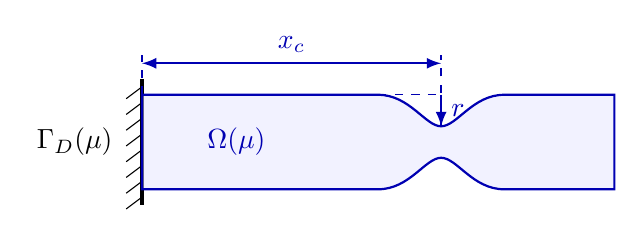
\begin{tikzpicture}[scale=1.0, >=stealth]
        % Styles
        \tikzset{
            deformed/.style={thick, draw=blue!70!black, fill=blue!10, fill opacity=0.5},
            dimension/.style={blue!70!black, <->, >=latex, line width=0.8pt},
            dimline/.style={blue!70!black, dashed, line width=0.5pt}
        }

        % Left Wall Hatching (Clamped Support)
        \draw[line width=1.5pt] (0,0.8) -- (0,-0.8);
        \foreach \y in {-0.7,-0.5,...,0.7} {
                \draw (0,\y) -- (-0.2,\y-0.15);
            }
        \node[left] at (-0.25, 0) {$\Gamma_D(\boldsymbol{\mu})$};

        % Parameterized Configuration \Omega(\boldsymbol{\mu})
        \draw[deformed] (0,0.6) -- (3.0,0.6) .. controls (3.4,0.6) and (3.6,0.2) .. (3.8,0.2) .. controls (4.0,0.2) and (4.2,0.6) .. (4.6,0.6) -- (6,0.6) -- (6,-0.6) -- (4.6,-0.6) .. controls (4.2,-0.6) and (4.0,-0.2) .. (3.8,-0.2) .. controls (3.6,-0.2) and (3.4,-0.6) .. (3.0,-0.6) -- (0,-0.6) -- cycle;
        \node[blue!70!black] at (1.2, 0.0) {$\Omega(\boldsymbol{\mu})$};

        % Dimension: x_c
        \draw[dimline] (0, 0.6) -- (0, 1.1);
        \draw[dimline] (3.8, 0.2) -- (3.8, 1.1);
        \draw[dimension] (0, 1.0) -- (3.8, 1.0) node[midway, above] {$x_c$};

        % Dimension: r
        \draw[dimline] (3.0, 0.6) -- (3.8, 0.6);
        \draw[blue!70!black, ->, >=latex, line width=0.8pt] (3.8, 0.6) -- (3.8, 0.2) node[midway, right] {$r$};
    \end{tikzpicture}
    \caption{Schematic of the parameterized notched cantilever beam configuration $\Omega(\boldsymbol{\mu})$ showing Dirichlet boundary support $\Gamma_D(\boldsymbol{\mu})$ and the design parameters $x_c$ (notch center position) and $r$ (notch radius).}
    \label{fig:notched_beam_geometry}
\end{figure}

\newpage


\section{Governing Equations \& Kinematics}
\enlargethispage{4\baselineskip}

\begin{figure}[htbp]
    \vspace{-0.4cm}
    \centering
    \makebox[\textwidth][c]{%
        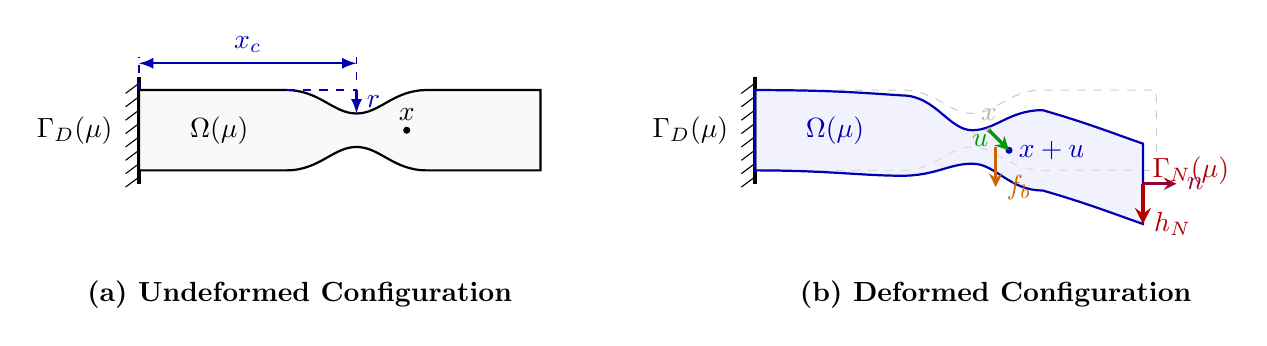
\begin{tikzpicture}[scale=0.85, >=stealth]
            % Styles
            \tikzset{
                reference/.style={thick, draw=black, fill=gray!5},
                deformed/.style={thick, draw=blue!70!black, fill=blue!10, fill opacity=0.5},
                dimension/.style={blue!70!black, <->, >=latex, line width=0.8pt},
                dimline/.style={blue!70!black, dashed, line width=0.5pt},
                force/.style={->, line width=1.5pt, red!70!black},
                displ/.style={->, line width=1.2pt, green!60!black}
            }

            % --- PANEL 1: UNDEFORMED CONFIGURATION ---
            \begin{scope}[xshift=0cm]
                % Left Wall Hatching (Clamped Support)
                \draw[line width=1.5pt] (0,0.8) -- (0,-0.8);
                \foreach \y in {-0.7,-0.5,...,0.7} {
                        \draw (0,\y) -- (-0.2,\y-0.15);
                    }
                \node[left] at (-0.25, 0) {$\Gamma_D(\boldsymbol{\mu})$};

                % Reference (Undeformed) Configuration \Omega(x_c)
                \draw[reference] (0,0.6) -- (2.2,0.6) .. controls (2.7,0.6) and (2.9,0.25) .. (3.25,0.25) .. controls (3.6,0.25) and (3.8,0.6) .. (4.3,0.6) -- (6,0.6) -- (6,-0.6) -- (4.3,-0.6) .. controls (3.8,-0.6) and (3.6,-0.25) .. (3.25,-0.25) .. controls (2.9,-0.25) and (2.7,-0.6) .. (2.2,-0.6) -- (0,-0.6) -- cycle;
                \node[black] at (1.2, 0.0) {$\Omega(\boldsymbol{\mu})$};

                % Dimension: x_c
                \draw[dimline] (0, 0.6) -- (0, 1.1);
                \draw[dimline] (3.25, 0.25) -- (3.25, 1.1);
                \draw[dimension] (0, 1.0) -- (3.25, 1.0) node[midway, above] {$x_c$};

                % Dimension: r
                \draw[dimline] (2.2, 0.6) -- (3.25, 0.6);
                \draw[blue!70!black, ->, >=latex, line width=0.8pt] (3.25, 0.6) -- (3.25, 0.25) node[midway, right] {$r$};

                % Point x
                \coordinate (X) at (4, 0.0);
                \fill[black] (X) circle (1.5pt) node[above] {$\vect{x}$};

                \node[below, font=\bfseries] at (2.4, -2.1) {(a) Undeformed Configuration};
            \end{scope}

            % --- PANEL 2: DEFORMED CONFIGURATION ---
            \begin{scope}[xshift=9.2cm]
                % Left Wall Hatching
                \draw[line width=1.5pt] (0,0.8) -- (0,-0.8);
                \foreach \y in {-0.7,-0.5,...,0.7} {
                        \draw (0,\y) -- (-0.2,\y-0.15);
                    }
                \node[left] at (-0.25, 0) {$\Gamma_D(\boldsymbol{\mu})$};

                % Light reference dashed contour
                \draw[dashed, gray!40] (0,0.6) -- (2.2,0.6) .. controls (2.7,0.6) and (2.9,0.25) .. (3.25,0.25) .. controls (3.6,0.25) and (3.8,0.6) .. (4.3,0.6) -- (6,0.6) -- (6,-0.6) -- (4.3,-0.6) .. controls (3.8,-0.6) and (3.6,-0.25) .. (3.25,-0.25) .. controls (2.9,-0.25) and (2.7,-0.6) .. (2.2,-0.6) -- (0,-0.6) -- cycle;

                % Parameterized Configuration \Omega(x_c)
                \draw[deformed]
                (0,0.6) .. controls (1.1,0.6) and (1.6,0.56) .. (2.2,0.52)
                .. controls (2.7,0.52) and (2.9,0.0) .. (3.25,0.0)
                .. controls (3.6,0.0) and (3.8,0.3) .. (4.3,0.3)
                .. controls (5.0,0.1) and (5.5,-0.1) .. (5.8,-0.2) --
                (5.8,-1.4)
                .. controls (5.5,-1.3) and (5.0,-1.1) .. (4.3,-0.9)
                .. controls (3.8,-0.9) and (3.6,-0.5) .. (3.25,-0.5)
                .. controls (2.9,-0.5) and (2.7,-0.68) .. (2.2,-0.68)
                .. controls (1.6,-0.68) and (1.1,-0.6) .. (0,-0.6) -- cycle;
                \node[blue!70!black] at (1.2, 0.0) {$\Omega(\boldsymbol{\mu})$};

                % Neumann Boundary \Gamma_N and Traction \vect{h}_N
                \node[right, red!70!black] at (5.8, -0.6) {$\Gamma_N(\boldsymbol{\mu})$};
                \draw[force] (5.8, -0.8) -- (5.8, -1.4) node[right] {$\vect{h}_N$};

                % Body Force \vect{f}_b
                \draw[->, line width=1.2pt, orange!80!black] (3.6, -0.25) -- (3.6, -0.85) node[right] {$\vect{f}_b$};

                % Outward normal vector \vect{n}
                \draw[->, line width=1.0pt, purple!80!black] (5.8, -0.8) -- (6.3, -0.8) node[right] {$\vect{n}$};

                % Kinematic point mapping
                \coordinate (X_ref) at (3.5, 0.0);
                \coordinate (x) at (3.8, -0.3);
                \fill[gray!60] (X_ref) circle (1.2pt) node[above, gray!60] {$\vect{x}$};
                \fill[blue!70!black] (x) circle (1.5pt) node[right] {$\vect{x} + \vect{u}$};
                \draw[displ] (X_ref) -- (x) node[midway, left] {$\vect{u}$};

                \node[below, font=\bfseries] at (3.6, -2.1) {(b) Deformed Configuration};
            \end{scope}

        \end{tikzpicture}%
    }


    \vspace{0.4cm}
    \small
    \begin{tabular}{ll}
        \toprule
        \textbf{Symbol}                      & \textbf{Description}                                                   \\
        \midrule
        $\Omega(\boldsymbol{\mu})$           & Parameterized physical configuration (depending on $\boldsymbol{\mu}$) \\
        $\Gamma_D(\boldsymbol{\mu})$         & Dirichlet boundary (clamped left edge where $\vect{u} = \vect{0}$)     \\
        $\Gamma_N(\boldsymbol{\mu})$         & Neumann boundary (surface under traction forces)                       \\
        $x_c$                                & Geometric parameter: notch longitudinal starting position              \\
        $r$                                  & Geometric parameter: radius of the symmetric notches                   \\
        $\vect{u}$                           & Displacement field vector $\vect{u}(\vect{x}, t; \boldsymbol{\mu})$    \\
        $\vect{h}_N$                         & Boundary traction load vector applied on $\Gamma_N(\boldsymbol{\mu})$  \\
        $\vect{f}_b$                         & Volumetric body force vector                                           \\
        $\vect{n}$                           & Outward unit normal vector to the boundary                             \\
        $\vect{x}$ and $\vect{x} + \vect{u}$ & Spatial coordinates in undeformed and deformed configurations          \\
        \bottomrule
    \end{tabular}
    \caption{Kinematic description and boundary conditions of the parameterized notched cantilever beam.}
    \label{fig:continuum_kinematics}
\end{figure}


The displacement field of the structure is denoted by $\vect{u}(\vect{x}, t; \boldsymbol{\mu})$ for $\vect{x} \in \Omega(\boldsymbol{\mu})$, and the stress state is represented by the Cauchy stress tensor $\boldsymbol{\sigma}$.
Assuming small strains and linear elastic isotropic material behavior, the strong form governing the transient response of the structural continuum on the parameterized physical domain $\Omega(\boldsymbol{\mu})$ over the time interval $(0, T]$ is given by the balance of linear momentum:
\begin{equation}
    \rho \ddot{\vect{u}} - \nabla \cdot \boldsymbol{\sigma}(\vect{u}) = \vect{f}_b \quad \text{in } \Omega(\boldsymbol{\mu}) \times (0, T]
\end{equation}
subject to the parameterized Dirichlet boundary conditions on $\Gamma_D(\boldsymbol{\mu})$ (fixed support at the left end) and Neumann boundary conditions on $\Gamma_N(\boldsymbol{\mu})$ (external loads applied to the boundaries):
\begin{align}
    \vect{u}                                     & = \vect{0} \quad \text{on } \Gamma_D(\boldsymbol{\mu}) \times (0, T]   \\
    \boldsymbol{\sigma}(\vect{u}) \cdot \vect{n} & = \vect{h}_N \quad \text{on } \Gamma_N(\boldsymbol{\mu}) \times (0, T]
\end{align}
along with the initial conditions at $t = 0$:
\begin{align}
    \vect{u}(\vect{x}, 0)       & = \vect{u}_0(\vect{x}) \quad \text{for } \vect{x} \in \Omega(\boldsymbol{\mu}) \\
    \dot{\vect{u}}(\vect{x}, 0) & = \vect{v}_0(\vect{x}) \quad \text{for } \vect{x} \in \Omega(\boldsymbol{\mu})
\end{align}
where $\rho$ is the material density, $\vect{f}_b$ is the body force vector, and $\vect{n}$ is the outward unit normal vector. The kinematic relation defines the linearized strain tensor $\boldsymbol{\varepsilon}(\vect{u})$ as:
\begin{equation}
    \boldsymbol{\varepsilon}(\vect{u}) = \frac{1}{2}\left(\nabla\vect{u} + (\nabla\vect{u})^T\right)
\end{equation}
For an isotropic material, the Cauchy stress tensor $\boldsymbol{\sigma}$ is related to the strain tensor via Hooke's law:
\begin{equation}
    \boldsymbol{\sigma}(\vect{u}) = \mat{D} \boldsymbol{\varepsilon}(\vect{u})
\end{equation}
where $\mat{D}$ is the constitutive matrix under Voigt notation.



\newpage
\section{Weak Formulation at the Continuum Level}
To derive the variational statement, we multiply the momentum balance equation by a test function $\delta\vect{u}$ belonging to the space of kinematically admissible variations:
\begin{equation}
    \mathcal{V}_0(\Omega(\boldsymbol{\mu})) = \{ \vect{v} \in [H^1(\Omega(\boldsymbol{\mu}))]^2 \mid \vect{v} = \vect{0} \text{ on } \Gamma_D(\boldsymbol{\mu}) \}
\end{equation}
Integrating by parts over the parameterized spatial domain $\Omega(\boldsymbol{\mu})$ yields the weak form:
\begin{equation}
    m(\ddot{\vect{u}}, \delta\vect{u}; \boldsymbol{\mu}) + k(\vect{u}, \delta\vect{u}; \boldsymbol{\mu}) = f(\delta\vect{u}) \quad \forall \delta\vect{u} \in \mathcal{V}_0(\Omega(\boldsymbol{\mu}))
\end{equation}
where the bilinear mass and stiffness forms, and the linear load form are defined respectively as:
\begin{align}
    m(\ddot{\vect{u}}, \delta\vect{u}; \boldsymbol{\mu}) & = \int_{\Omega(\boldsymbol{\mu})} \rho \ddot{\vect{u}} \cdot \delta\vect{u} \, d\Omega                                                                      \\
    k(\vect{u}, \delta\vect{u}; \boldsymbol{\mu})        & = \int_{\Omega(\boldsymbol{\mu})} \boldsymbol{\varepsilon}(\delta\vect{u})^T \mat{D} \boldsymbol{\varepsilon}(\vect{u}) \, d\Omega                          \\
    f(\delta\vect{u})                                    & = \int_{\Omega(\boldsymbol{\mu})} \vect{f}_b \cdot \delta\vect{u} \, d\Omega + \int_{\Gamma_N(\boldsymbol{\mu})} \vect{h}_N \cdot \delta\vect{u} \, d\Gamma
\end{align}



\section{Shape Parameterization Challenge and Mappings}
For shape-parametric structural mechanics, a key challenge is that the physical domain $\Omega(\boldsymbol{\mu})$ varies with the design parameter vector $\boldsymbol{\mu}$. When performing numerical simulation across different configurations, this geometric variation introduces two major bottlenecks:
\begin{enumerate}
    \item \textbf{Vector Space Incompatibility:} Since the geometry changes shape, the discretization grids (or element nodes) vary, meaning that displacement snapshots collected across different parameter configurations do not live in the same vector space. This prevents Proper Orthogonal Decomposition (POD) and Singular Value Decomposition (SVD) from being performed directly in the physical space.
    \item \textbf{Online Assembly Overhead:} If the physical geometry is directly remeshed for each parameter change (the naive approach), the global system matrices must be fully assembled and integrated online, which is computationally expensive and prohibits real-time simulation.
\end{enumerate}

To resolve these compatibility and computational issues, two main strategies exist:
\begin{itemize}
    \item \textbf{Physical Remeshing and Interpolation:} Re-discretizing the deforming domain and interpolating fields between meshes. This approach is topologically inconsistent, computationally heavy, and prone to interpolation errors.
    \item \textbf{Reference Configuration Mapping (Pullback):} Defining a fixed, parameter-independent reference configuration $\hat{\Omega}$ (or parent parametric space $\hat{\Omega}_{\text{param}}$) and pulling all physical fields, gradients, and integrals back to it. This approach retains a constant discretization topology and shifts all parameter dependencies into the integration Jacobians.
\end{itemize}

In this work, the diffeomorphic pullback mapping approach is chosen because it establishes a mathematically consistent framework where all snapshot vectors lie in a single, fixed vector space, enabling projection-based model reduction. The mathematical details of this pullback mapping at both the continuum and discretized levels, along with its implementation, are discussed in detail in Chapter \ref{ch:pullback}.

\section{Summary}
In this chapter, we established the mathematical framework for the parameterized continuum model of the notched cantilever beam on the parameterized physical domain $\Omega(\boldsymbol{\mu})$. We formulated the strong-form governing equations and derived the corresponding weak variational statement. We also identified the domain compatibility challenge associated with shape variations and motivated the need for a reference configuration mapping. In the next chapter, we will discretize the spatial domain using Isogeometric Analysis (IGA) before detailing the mathematical formulation of the pullback mapping and its numerical integration in Chapter \ref{ch:pullback}.
